%%% NOTE: I AM FIRST COMPILING MY TEX FILE IN VS Code; WILL TRANSFER CONTENT


% **Presentation Structure:**

% 1) Introduction: Problem Statement and Motivation
% 	- Why the problem is relevant; particular aspect we focus on (crossover disambiguation in sequential memory);
% 	- Goal
% 	- Quickly introduce the model we hope to implement; introduce idea of energetic approach
% 2) Lit Review
% 	* Important papers in the fields (including Krotov on DAM)
% 	* Clear Gap: no learning rules for disambiguation of crossover
% 3) Introduction of Model
% 	* Motivation for Kuramoto in a Hopfield Network (mention what we are hoping to observe: smoothness when retrieving, and mention importance to physical oscillator-based simulators)
% 	* Introduce basic learning rule (derived for Kuramoto from Krotov DAM) and algorithm for sequence retrieval; display graph for single sequence retrieval
% 	* Demonstrate the inability of the basic rule to resolve branching / crossover
% 	* Using argument on the innate symmetry of the energy landscape, introduce heterogeneous learning rules + motivation/reasoning
% 4) Experiment
% 	* Set up benchmarks
% 	* Table display of learning rules
% 	* Define experiment conditions; important global parameters
% 	* Experimental results, including superposition of learning rules
% 	* Display robustness, sweeping across different corruption ratios and N
% 	* Discussion: based on this talk about which learning rules perform better + limitations
% 5) Analytical Part (Jona)
% 	* Tensor notation: symmetric and asymmetric components
% 	* Scalability?
% 6) Conclusion + Applications
% 	* Quick notes on implementation into physical simulator and problems that this can solve (include those in Neurobiology?)


% UNSURE: in which order, benchmark first and then new learning rule or benchmark in section on experiment 

%%% NOTE: I AM FIRST COMPILING MY TEX FILE IN VS Code; WILL TRANSFER CONTENT

% =====================================================================
%  Crossover disambiguation in Kuramoto-coupled dense associative
%  sequential memory.
%
%  Deck structure (as built):
%    1  Introduction   -- crossover problem; Hebbian -> Krotov DAM ->
%                         Kuramoto sequence drive; asymmetric couplings
%                         give a Lyapunov function, NOT an energy
%    2  Literature     -- foundations; the open problem
%    3  Model          -- baseline rule + algorithm; its failure at a
%                         crossover; symmetry of the Lyapunov function;
%                         heterogeneous lag-context rules
%    4  Results        -- benchmarks, catalogue, conditions, crossover
%                         resolution, superposition, robustness,
%                         findings I (rules) and II (dynamics/scaling)
%    5  Analysis       -- tensor decomposition; scalability      [Jona]
%    6  Conclusions    -- main result; applications
%    7  Open questions -- physical implementation; decaying neurons;
%                         randomly generated sequences
%
%  Remaining \TODO{} placeholders mark numbers and figures to drop in
%  from the executed notebooks.
% =====================================================================

\documentclass[aspectratio=169]{beamer}

\usetheme{Madrid}
\usecolortheme{default}

\usepackage[utf8]{inputenc}
\usepackage{amsmath, amssymb}
\usepackage{booktabs}
\usepackage{graphicx}
\graphicspath{{../}{./}}
\usepackage{algorithm}
\usepackage{algpseudocode}
\usepackage{tikz}
\usetikzlibrary{arrows.meta, positioning}

% Convenience macros used throughout (edit to taste)
\newcommand{\xxi}{\xi}
\newcommand{\thetavar}{\theta}
\newcommand{\mvar}{m}
\newcommand{\TODO}[1]{{\color{red}\textbf{[TODO: #1]}}}
% Figure title: a short scientific label placed under each plot, above its caption.
\newcommand{\figtitle}[1]{\\[1mm]{\footnotesize\textbf{#1}}\\[1mm]}

\title[Kuramoto DAM: Crossover Disambiguation]{Crossover Disambiguation in Kuramoto-Coupled\\ Dense Associative Sequential Memory}
\subtitle{Learning rules for resolving branch ambiguity in phase-oscillator sequence retrieval}
\author[D. Vorobiev \and J. N\"agerl]{Daniel Vorobiev \and Jona N\"agerl}
\institute{University of Cambridge}

\begin{document}

\begin{frame}
  \titlepage
\end{frame}

\begin{frame}{Outline}
  \tableofcontents
\end{frame}


% =====================================================================
\section[Introduction]{Introduction and Motivation}
% =====================================================================

\begin{frame}{Sequential associative memory}
  \begin{itemize}
    \item Hopfield memories store \emph{static} attractors. Motor sequences,
      speech and episodic replay require \emph{ordered} ones.
    \item Sequential retrieval $=$ a chain of transitions $\mu \to \mu+1$.
    \item \TODO{one line: hippocampal replay + phase-native hardware}
  \end{itemize}
\end{frame}

\begin{frame}{The crossover problem}
  \begin{columns}
    \begin{column}{0.55\textwidth}
      \begin{itemize}
        \item Two sequences share a contiguous run of patterns.
        \item At the shared state the network configuration is
          \emph{identical} either way: the history is not encoded in the state.
        \item Markov-1 drives both continuations equally, so noise alone
          picks the branch.
      \end{itemize}
      \vspace{2mm}
      \centering\textbf{Can the coupling alone encode the route into $\xxi^0$?}
    \end{column}
    \begin{column}{0.45\textwidth}
      \centering
      \begin{tikzpicture}[node distance=10mm, >=Stealth]
        \node (m1) {$M_1$};
        \node (x0) [right=of m1] {$\xxi^0$};
        \node (m2) [above right=6mm and 10mm of x0] {$M_2$};
        \node (m4) [below right=6mm and 10mm of x0] {$M_4$};
        \draw[->] (m1) -- (x0);
        \draw[->, dashed, red] (x0) -- (m2) node[midway, above] {?};
        \draw[->, dashed, red] (x0) -- (m4) node[midway, below] {?};
      \end{tikzpicture}
    \end{column}
  \end{columns}
\end{frame}

\begin{frame}{Objectives}
  \begin{enumerate}
    \item A Kuramoto phase-oscillator DAM for \emph{sequences}.
    \item A learning rule that resolves crossover from the coupling alone
      --- no external gating signal.
    \item \emph{When} is disambiguation possible at all, and how robust is
      it to corruption, network size and disorder?
    \item \TODO{one line: analytical / tensor contribution}
  \end{enumerate}
\end{frame}

\begin{frame}{From Hebbian storage to dense associative memory}
  \begin{columns}[T]
    \begin{column}{0.5\textwidth}
      \textbf{Hopfield (1982)} --- pairwise Hebbian
      $J_{ij} = \frac{1}{N}\sum_\mu \xxi_i^\mu \xxi_j^\mu$:
      \[
        E = -\tfrac{N}{2}\sum_\mu \bigl(\mvar^\mu\bigr)^2 ,\quad
        \mvar^\mu = \tfrac1N \sum_j \xxi^\mu_j s_j
      \]
      Crosstalk caps capacity at $\approx 0.14N$.
    \end{column}
    \begin{column}{0.5\textwidth}
      \textbf{Krotov--Hopfield DAM (2016)} --- sharpen the nonlinearity,
      i.e.\ higher-order interactions:
      \[
        E = -\sum_\mu F\bigl(\mvar^\mu\bigr), \quad F(x) = x^{\,d+1}
      \]
      Capacity $\mathcal{O}(N^{d})$; minima sharpen with $d$.
    \end{column}
  \end{columns}
  \vspace{3mm}
  \begin{block}{Resulting drive}
    Descending $E$ gives the \emph{pure-power} drive
    $\sum_\mu \xxi_i^\mu (\mvar^\mu)^{d}$ --- one pattern index per term,
    exponent $d$ as in Krotov DAM. Every rule that follows changes only
    \emph{which} pattern each factor reads.
  \end{block}
\end{frame}

\begin{frame}{From the DAM energy to the Kuramoto sequence drive}
  \begin{enumerate}
    \item \textbf{Spins $\to$ phases:} $s_i = \cos\thetavar_i$, so
      $\dot\thetavar_i = -\partial_{\thetavar_i} E
       = \omega_i - \sin\thetavar_i \sum_\mu \xxi_i^{\mu}(\mvar^\mu)^d$.
    \item \textbf{Symmetric ($\mu \to \mu$):} true gradient flow; stored
      patterns are minima.
    \item \textbf{Asymmetric ($\mu \to \mu+1$):} drive the \emph{successor}
      (Sompolinsky--Kanter): stored patterns cease to be resting points and
      the state traverses the chain.
  \end{enumerate}
  \begin{alertblock}{Absence of an energy functional}
    Asymmetric couplings $\Rightarrow$ no potential with
    $\dot{\thetavar} = -\nabla E$. ``Minima'', ``saddles'', ``symmetry of
    the landscape'' below refer to a \textbf{Lyapunov function} of the flow.
    The absence of gradient structure is precisely what permits transitions.
  \end{alertblock}
\end{frame}


% =====================================================================
\section{Literature Review}
% =====================================================================

\begin{frame}{Foundations}
  \begin{itemize}
    \item \textbf{Hopfield (1982)} --- pairwise Hebbian attractor memory.
    \item \textbf{Krotov \& Hopfield (2016)} --- dense associative memory:
      power-$d$ interactions, super-linear capacity.
    \item \textbf{Sompolinsky \& Kanter (1986)} --- asymmetric
      $\mu \to \mu+1$ couplings turn attractors into a sequence.
    \item \textbf{Kuramoto (1975)} --- the phase-oscillator substrate.
    \item \textbf{N\"agerl \& Berloff (2025)}, arXiv:2507.21984 --- DAM in a
      higher-order Kuramoto network; the base model for this work.
    \item \TODO{oscillator / photonic hardware refs; Markov-chain sequence refs}
  \end{itemize}
\end{frame}

\begin{frame}{Open problem: crossover disambiguation}
  \begin{block}{No learning rule for crossover disambiguation}
    Existing formalisms specify \emph{how} one pattern drives the next, but
    not what happens when two sequences pass through the \emph{same} state.
  \end{block}
  \begin{itemize}
    \item A transition matrix only ever sums pure powers,
      $\sum_\beta T_{\alpha\beta}(\mvar^\beta)^d$.
    \item It cannot represent a conjunction: \emph{drive $\xxi^{\mu+1}$ only
      if $\mvar_\mu$ \textbf{and} $\mvar_{\mu-1}$ are simultaneously large.}
    \item $\Rightarrow$ gate on a \emph{product of overlaps at different
      lags}.
  \end{itemize}
\end{frame}


% =====================================================================
\section[Model]{Model and Learning Rules}
% =====================================================================

\begin{frame}{Motivation for Kuramoto dynamics}
  \begin{itemize}
    \item \textbf{Smooth retrieval.} Continuous phases resolve the traversal of a
      crossover \emph{in time}, rather than as a discrete jump.
    \item \textbf{Physical realizability.} Rules expressed purely as oscillator
      coupling are natively executable on analog and photonic hardware.
    \item \TODO{theta--gamma phase coding, if used in Applications}
  \end{itemize}
\end{frame}

\begin{frame}{Objects: patterns, overlaps, couplings}
  \centering
  \small
  \begin{tabular}{lll}
    \toprule
    Object & Shape & Content \\
    \midrule
    $\thetavar$            & $N$         & oscillator phases; $s_i = \cos\thetavar_i$ \\
    $\xxi^{a,\mu}$         & $K \times P \times N$ & stored patterns,
      $\xxi_i = \cos\varphi_i \in \{-1,+1\}$, $\varphi_i \in \{0,\pi\}$ \\
    $\xxi^{a,\mu+1}$       & $K \times P \times N$ & successor tensor: row $\mu$ holds
      the pattern $\mu$ drives \\
    $\mvar_i^{a,\mu}$      & $K \times P$ (per $i$) & leave-one-out overlaps,
      $\frac{1}{N-1}\sum_{j \ne i}\xxi_j^{a,\mu}\cos\thetavar_j$ \\
    $T^a_{\alpha\beta}$    & $K \times P \times P$ & transition matrix; row $=$
      destination, column $=$ source \\
    $R$ (rule table)       & $n_{\text{terms}} \times (d+2)$ &
      rows $[\,s \mid \ell_1 \dots \ell_d \mid w\,]$: target offset, lags, weight \\
    $J$ (coupling)         & rank $d+1$  & $J_i^{\mu_1 \dots \mu_d,\,\nu}$, contracted
      against $d$ overlaps \\
    \bottomrule
  \end{tabular}
  \\[3mm]
  \begin{itemize}
    \item Patterns are real, so $|\mvar|^2 = \mvar^2$: the write-up's fourth-order
      bidegree-$(2,1)$ fields are the $d = 3$ rows of $R$.
    \item $T$ sums \emph{pure powers} $\sum_\beta T_{\alpha\beta}(\mvar^\beta)^d$;
      a rule table multiplies overlaps read at \emph{different} lags, which no $T$ can
      express. The shift matrix $T_{\alpha\beta} = \delta_{\alpha,\beta+1}$ and the row
      $[\,1 \mid 0,0,0 \mid 1\,]$ are the same baseline.
  \end{itemize}
\end{frame}


\begin{frame}{Baseline rule and retrieval algorithm}
  \[
    \dot\thetavar_i = \omega_i - \sin\thetavar_i \sum_\mu
      \xxi_i^{\mu+1}\,\bigl(\mvar_i^{\mu}\bigr)^{d}, \qquad
      \mvar_i^{\mu} = \frac{1}{N-1}\sum_{j\ne i}\xxi_j^{\mu}\cos\thetavar_j
  \]
  \begin{center}
    \small Read the current overlap, drive the next pattern:
    Sompolinsky--Kanter at Krotov power $d$.
  \end{center}
  \begin{algorithm}[H]
    \small
    \begin{algorithmic}[1]
      \State cue $\thetavar(0) \gets$ (possibly corrupted) $\xxi^{0}$
      \For{each step}
        \State $\mvar^\mu_i$ for all $\mu$; \; $V_i = \sum_\mu \xxi_i^{\mu+1}(\mvar_i^\mu)^d$
        \State $\thetavar_i \mathrel{+}= dt\,(\omega_i - \sin\thetavar_i V_i)$ \; ($+$ noise)
      \EndFor
      \State decode the sequence from overlap peaks
    \end{algorithmic}
  \end{algorithm}
\end{frame}

\begin{frame}{Single-sequence retrieval, baseline rule}
  \centering
  
\includegraphics[height=0.68\textheight,width=\textwidth,keepaspectratio]{outputs/output.png}
  \figtitle{Pattern overlaps $\mvar^\mu(t)$ during single-chain retrieval under the baseline (\texttt{forward}) rule}
  {\small \TODO{caption: clean peak-to-peak retrieval through $P$ patterns}}
\end{frame}

\begin{frame}{Baseline rule at a crossover}
  \centering
  
\includegraphics[height=0.62\textheight,width=0.8\textwidth,keepaspectratio]{outputs/crossover_vanilla.png}
  \figtitle{Branch overlaps out of the shared state at a crossover, baseline (\texttt{forward}) rule}
  {\small Both continuations rise together out of the shared state.
  Branch choice at chance: \TODO{XX\%} vs.\ $50\%$.}
\end{frame}

\begin{frame}{Innate symmetry of the Lyapunov function}
  \begin{itemize}
    \item Couplings are asymmetric $\Rightarrow$ no energy; the flow is
      organized by a Lyapunov function $V$ built from the same pure powers.
    \item Every term of $V$ reads \emph{one} pattern index --- nothing in it
      records \emph{how} the state reached the shared pattern.
    \item At $\xxi^\star$ the gate depends only on $\mvar(\xxi^\star)$, identical
      for both branches: the two exits are related by an exact symmetry of
      $V$ (a degenerate saddle).
    \item[$\Rightarrow$] The symmetry must be broken by information the
      current state cannot carry: overlaps at \emph{several lags},
      multiplied rather than summed within a single term.
  \end{itemize}
\end{frame}

\begin{frame}{Heterogeneous lag-context rules}
  \[
    \dot\thetavar_i = \omega_i - \sin\thetavar_i \sum_{\mu}\sum_{\text{terms}}
      w \;\xxi_i^{\mu+s} \prod_{l \in \text{lags}} \mvar_i^{\mu - l}
  \]
  \begin{itemize}
    \item A rule is a \emph{table of terms}: target offset $s$, $d$ source
      lags, weight $w$. Lags $(0,0,0)$ recovers the forward rule.
    \item Different lags in one term $\Rightarrow$ the gate encodes
      \emph{which branch} produced the current state.
  \end{itemize}
\end{frame}


% =====================================================================
\section[Results]{Numerical Experiments and Results}
% =====================================================================
%  Structure mirrors results_summary.ipynb:
%    1 why anything moves      2 why branching is hard
%    3 metrics / topologies / statistics
%    4 robustness              5 appendix
%  Figures: presentation/figures/, generated by that notebook.
% =====================================================================

\begin{frame}{How the experiments are organised}
  \begin{enumerate}
    \item \textbf{Why anything moves.} $\omega \equiv 0$ is an exact fixed point;
      the natural frequency is what starts the cascade, and how much of it matters.
    \item \textbf{Why branching is hard.} A shared run is bit-identical between
      branches; the gate must reach past it.
    \item \textbf{Metrics, topologies, statistics.} Four crossover metrics, four
      geometries, $100$-instance seed sweeps with spread.
    \item \textbf{Robustness.} Network size, corruption ratio, and two knobs on the drive.
    \item \textbf{Appendix.} Random patterns; settle vs.\ loop.
  \end{enumerate}
  \vspace{2mm}
  {\small Every number below is reproduced by \texttt{results\_summary.ipynb}.}
\end{frame}

\begin{frame}{Sequence construction: smooth corruption chains}
  \begin{columns}[T]
    \begin{column}{0.56\textwidth}
      \begin{itemize}
        \item $\xxi^{1}$ uniform on $\{0,\pi\}^N$; then
          $\xxi^{k+1} = \mathrm{corrupt}(\xxi^{k},\rho)$: $\lfloor \rho N \rfloor$ sites
          drawn without replacement, $\varphi \to \pi - \varphi$.
        \item Consecutive overlap is therefore fixed by construction:
          \[
            \tfrac1N \textstyle\sum_i \xxi^{k}_i \xxi^{k+1}_i = 1 - 2\rho,
            \qquad d(\xxi^k,\xxi^{k+1}) = 2\rho .
          \]
        \item The patterns form a \emph{chain}: neighbours stay inside each
          other's basin, which is what lets the cascade hop at all.
        \item Lagged overlaps decay geometrically,
          $\mvar_{\mu-\ell} \sim (1-2\rho)^{\ell}$: hence the gain filter's
          $(1-2\rho)^{-\sum\text{lags}}$.
      \end{itemize}
    \end{column}
    \begin{column}{0.44\textwidth}
      \centering
      \begin{tikzpicture}[node distance=6mm, >=Stealth, font=\scriptsize]
        \node (a1) {$\xxi^{A,1}$};
        \node (a2) [right=of a1] {$\xxi^{A,2}$};
        \node (s)  [right=of a2] {$\boxed{\xxi^{\star}}$};
        \node (a4) [above right=4mm and 7mm of s] {$\xxi^{A,4}$};
        \node (b4) [below right=4mm and 7mm of s] {$\xxi^{B,4}$};
        \node (b2) [below left=11mm and 0mm of a2] {$\xxi^{B,2}$};
        \node (b1) [left=of b2] {$\xxi^{B,1}$};
        \draw[->] (a1) -- (a2); \draw[->] (a2) -- (s);
        \draw[->] (b1) -- (b2); \draw[->] (b2) -- (s);
        \draw[->] (s) -- (a4); \draw[->] (s) -- (b4);
      \end{tikzpicture}
      \\[2mm]
      {\scriptsize Shared run generated \emph{once} and reused by both branches: those
      overlaps are bit-identical, so the ambiguity is exact. Each branch is an
      independent corruption chain off the run.}
      \\[2mm]
      {\scriptsize Uncorrelated patterns score $0\%$ for every rule --- nothing
      retrieves without the chain.}
    \end{column}
  \end{columns}
\end{frame}


\begin{frame}{Benchmarks}
  \centering
  \small
  \begin{tabular}{llccl}
    \toprule
    Tag & Geometry & $P$ & Shared run $L$ & Reach needed \\
    \midrule
    \texttt{2-1-2} & one shared pattern   & 5 & 1 & 1 \\
    \texttt{2-2-2} & shared segment       & 6 & 2 & 2 \\
    \texttt{2-3-2} & failure case         & 7 & 3 & 3 (beyond catalogue) \\
    \bottomrule
  \end{tabular}
  \\[3mm]
  \begin{itemize}
    \item \textbf{Scoring:} every \emph{unshared} pattern of the cued branch
      decoded, in order. Shared positions carry no rule information and are
      excluded.
    \item \textbf{Branch diagnostic:} correct vs.\ incorrect drive at the
      exit; separates incorrect selection from correct selection without
      lock-on.
  \end{itemize}
\end{frame}

\begin{frame}{Metrics used throughout}
  \centering\scriptsize
  \begin{tabular}{llp{5.9cm}l}
    \toprule
    & metric & definition & chance / floor \\
    \midrule
    \multicolumn{4}{l}{\textbf{Crossover} --- \texttt{2-1-2}, \texttt{2-2-2}, \texttt{2-3-2}; shared positions excluded} \\
    \midrule
    1 & \texttt{correct}        & every unshared pattern of the cued branch decoded \emph{in order}, before the other branch appears & --- \\
      & \texttt{crossed}        & the other branch appears first & --- \\
      & \texttt{incomplete}     & the run ended before the branch resolved & --- \\
    2 & overlap quality         & mean peak overlap of those patterns, successful attempts only, with spread & --- \\
    3 & \textbf{branch-correct} & did the trajectory favour the cued continuation? & $0.5$ \\
    4 & margin                  & signed gap between the cued and the other continuation's peak overlap & $0$ \\
    \midrule
    \multicolumn{4}{l}{\textbf{Single chain} --- $P = 10$, no branch} \\
    \midrule
    5 & retrieval fraction      & how much \emph{of a} sequence came back; partial credit on a strict prefix & $1/P = 0.10$ \\
    6 & strict rate             & how many \emph{of the} sequences came back whole & --- \\
    \bottomrule
  \end{tabular}
  \\[2mm]
  \begin{itemize}\scriptsize
    \item A pattern counts as decoded at overlap $\ge$ \texttt{tolerance} $= 0.5$.
    \item \textbf{Metric 3 isolates the decision}; metric 1 bundles it with completion,
      $\text{correct} \approx \text{branch-correct} \times (1 - \text{incomplete})$.
    \item \texttt{self} is the control in both regimes, and \texttt{forward} the baseline at a crossover.
  \end{itemize}
\end{frame}

\begin{frame}{Catalogue of learning rules}
  \centering
  \small
  \begin{tabular}{lll}
    \toprule
    Rule & Gate at pattern $\mu$ & Reach \\
    \midrule
    \texttt{self} & $\xxi^\mu \mvar_\mu^3$ & 0 (control) \\
    \texttt{forward} (baseline) & $\xxi^{\mu+1} \mvar_\mu^3$ & 0 \\
    \texttt{skip-two} & $\xxi^{\mu+2} \mvar_\mu^3$ & 0 \\
    \texttt{bigram} & $\xxi^{\mu+1} \mvar_\mu |\mvar_{\mu-1}|^2$ & 1 \\
    \texttt{multilag} & $\xxi^{\mu+1} \mvar_\mu \sum_k w_k |\mvar_{\mu-k}|^2$ & $\le K$ \\
    \texttt{coh bigram} & $\xxi^{\mu+1} \mvar_\mu^2 \mvar_{\mu-1}$ & 1 \\
    \texttt{coh trigram} & $\xxi^{\mu+1} \mvar_\mu \mvar_{\mu-1} \mvar_{\mu-2}$ & 2 \\
    \bottomrule
  \end{tabular}
  \\[3mm]
  {\small Reach $\ge L$ is the entry requirement for accessing \emph{any} unshared
  information. Clearing it does not guarantee the rule can use it.}
\end{frame}
\begin{frame}{Global parameters}
  \centering
  \footnotesize
  \begin{tabular}{llll}
    \toprule
    Symbol & Value & Symbol & Value \\
    \midrule
    $N$             & $200$ crossover; $100$ single (swept) & $dt$          & $0.05$ \\
    $P$             & $5,6,7$ crossover; $10$ single      & $T$             & $80$ crossover; $180$ single \\
    $d$             & $3$                                 & integrator      & Euler / Euler--Maruyama \\
    $\rho$          & $0.2$ (sweep $0.05$--$0.35$)        & early stop      & $\max_i|\dot\thetavar_i| < 10^{-6}$, $10$ steps \\
    $\mu_\omega$    & $0$                                 & tolerance       & $0.5$ overlap to decode a pattern \\
    $\sigma_\omega$ & $0.3$                               & decoder margin  & $0.01$ crossover; $10^{-3}$ single \\
    phase noise     & $0.01$ (inert: ODE mode)            & dwell           & $20$ per transition \\
    trials          & $20 \times 2$ cues; $100$ seed sweep & seeds          & pool of $10^4$ \\
    \bottomrule
  \end{tabular}
  \\[3mm]
  \begin{itemize}
    \item $\omega \neq 0$ is load-bearing --- see next slide.
    \item Raw and gain-corrected catalogues are run at every operating point;
      the gain is rebuilt at each $\rho$ of a sweep.
    \item \textbf{Two base sizes.} Branch choice saturates at $N = 200$, so the crossover
      experiments run there. The single-chain sweeps keep $N = 100$ as their base and sweep
      $N$ explicitly --- that sweep \emph{is} the experiment.
    \item \textbf{Caveat:} every network uses \texttt{seed=10}, so one $\omega$
      draw is reused throughout. On the $\omega$ axis every result is $n = 1$.
  \end{itemize}
\end{frame}

% ---------------------------------------------------------------- 1
\begin{frame}{1. Why anything moves: the natural frequency}
  \centering
  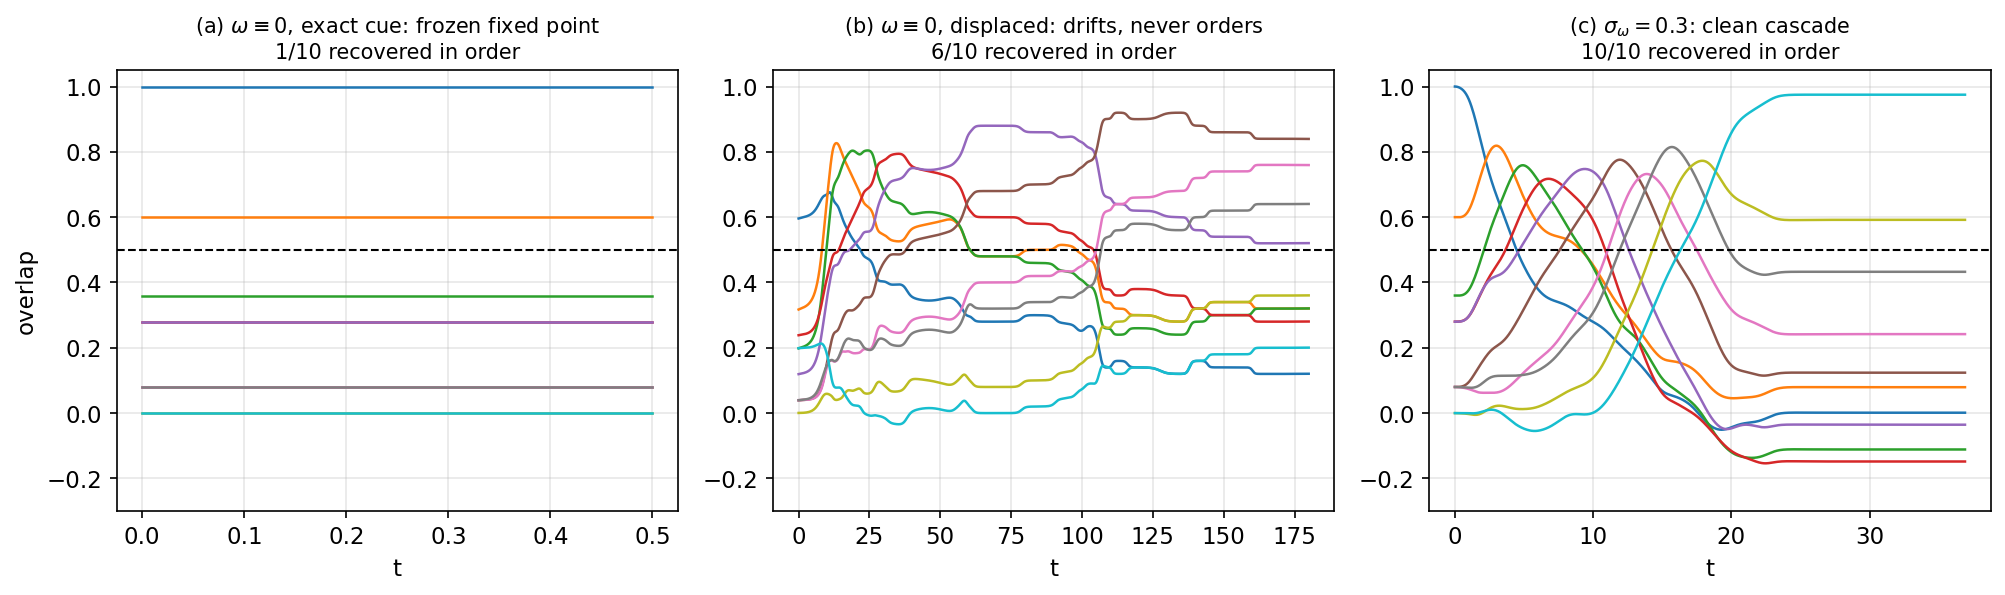
\includegraphics[width=\textwidth,height=0.45\textheight,keepaspectratio]{figures/fig01_stall.png}
  \figtitle{Retrieval at $\omega \equiv 0$ from an exact cue (a) and a displaced cue (b), against $\sigma_\omega = 0.3$ (c)}
  {\scriptsize Note the differing time axes: (a) exits at the stationary early-stop within a
  few steps.}
  \begin{itemize}\small
    \item At an exact cue every $\thetavar_i \in \{0,\pi\}$, so $\sin\thetavar_i = 0$ and the
      coupling $-\sin\thetavar_i V_i$ vanishes \emph{identically}, however large $V_i$ is.
      \textbf{(a)} sits at an exact fixed point --- the drive is degenerate. The $1/10$ it
      scores is the cue itself.
    \item \textbf{(b)} displaced start (flips \emph{plus} angular jitter, 
      off-lattice). No reliable cascade.
    \item \textbf{(c)} $\sigma_\omega = 0.3$: a clean cascade, each pattern peaking in turn and
      the full chain recovered in order.
  \end{itemize}
\end{frame}

\begin{frame}{1. How much frequency? The usable band}
  \centering
  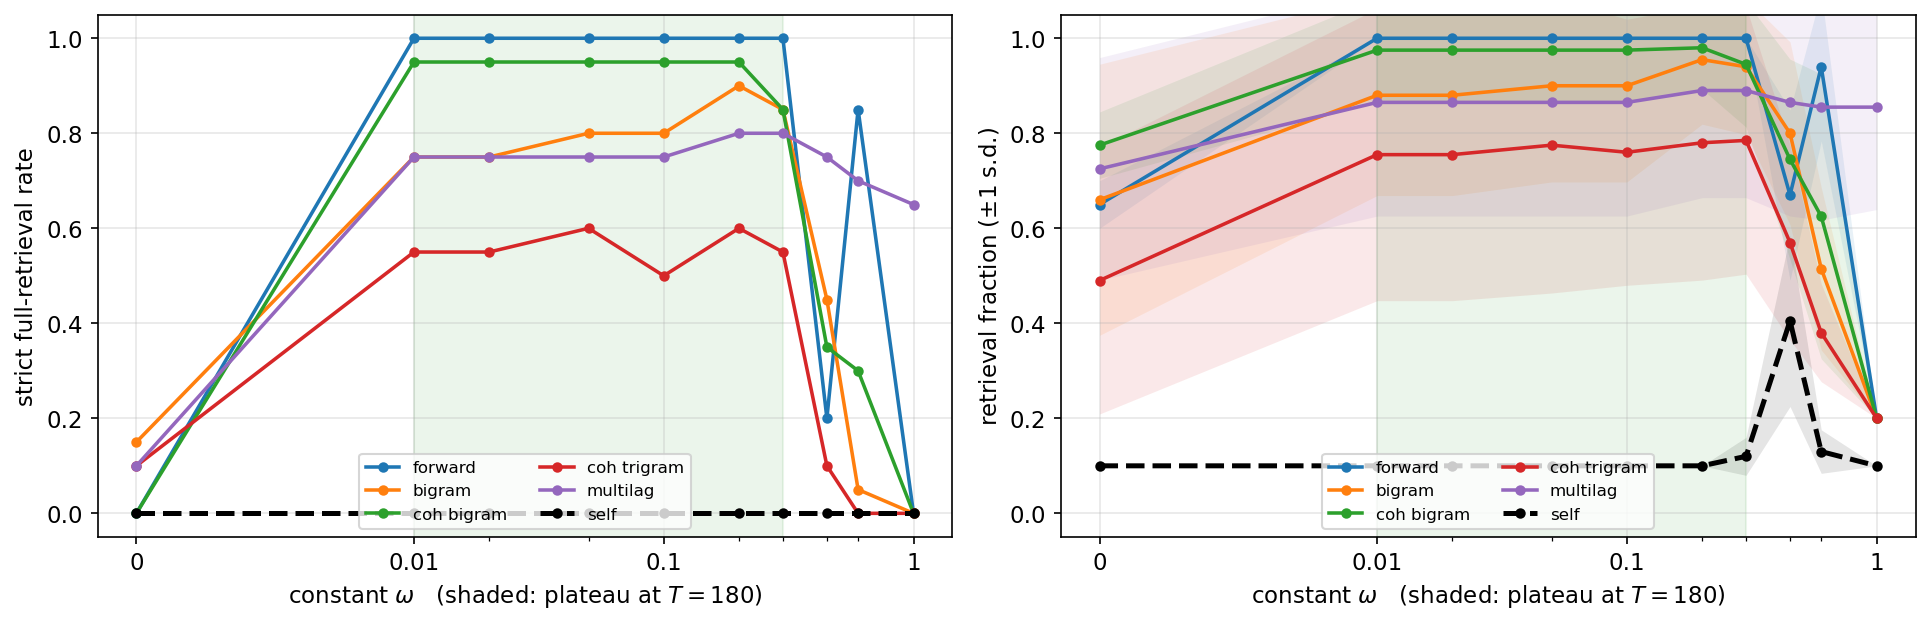
\includegraphics[width=\textwidth,height=0.43\textheight,keepaspectratio]{figures/fig02_omega_band.png}
  \figtitle{Retrieval fraction against $\omega$ at $T = 54$ and $T = 180$, by learning rule}
  \begin{itemize}\small
    \item $\omega = 0$ is \textbf{singular}: at an exact cue it is a fixed point, and any
      $\varepsilon > 0$ already sits in a different regime.
    \item A rotating frame \textbf{cannot} absorb a uniform $\omega$ here --- the drive is
      anchored to the absolute $\{0,\pi\}$ lattice, so the frame shift survives in the dynamics.
    \item At high $\omega$ ($\approx 1$) the drive is overwhelmed by the natural frequency: the
      overlaps never peak and noise is dominant. The usable band is $\sigma_\omega \in [0.1,0.5]$.
  \end{itemize}
\end{frame}

% ---------------------------------------------------------------- 2
\begin{frame}{2. Why branching is hard, and what fixes it}
  \centering
  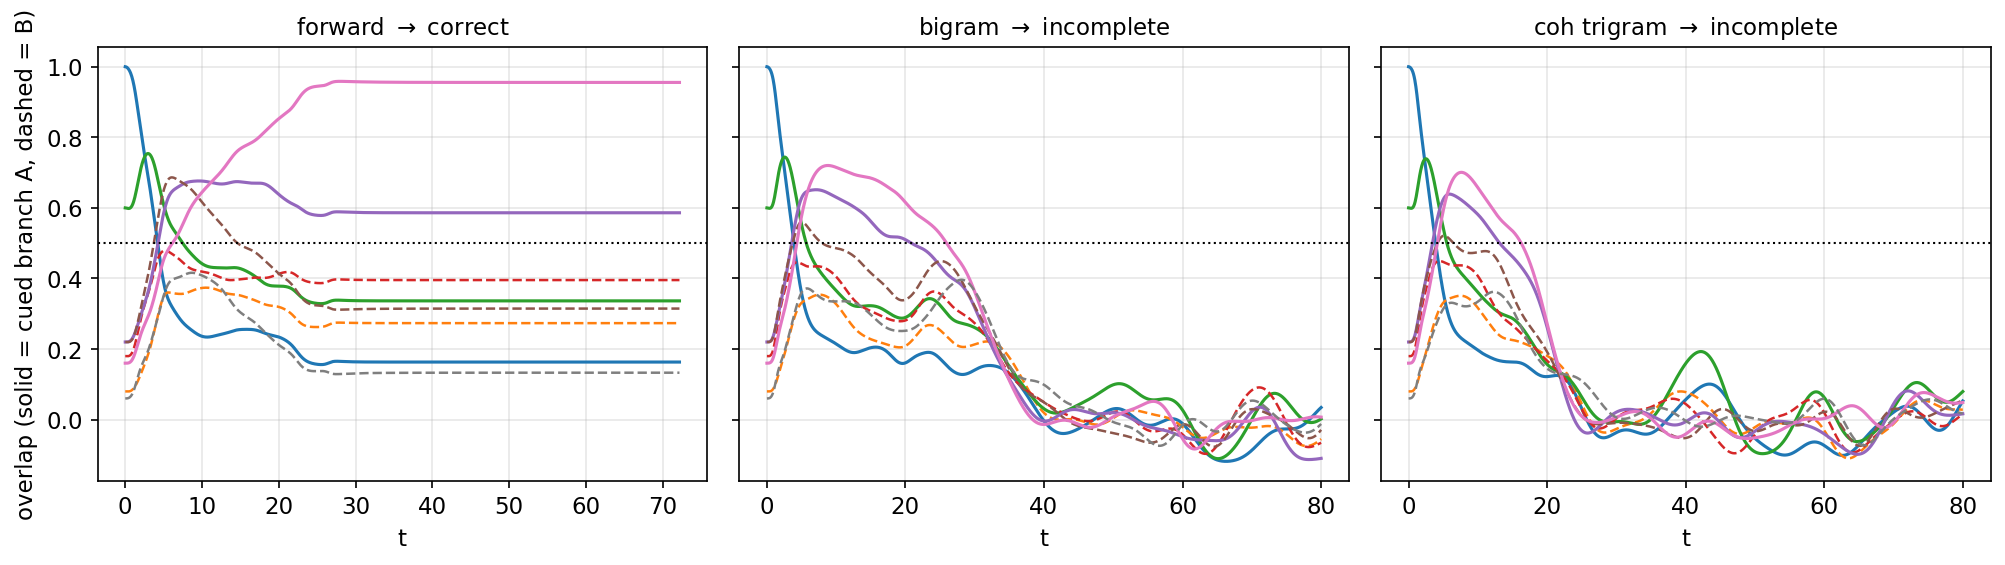
\includegraphics[width=\textwidth,height=0.39\textheight,keepaspectratio]{figures/fig03_crossover_traces.png}
  \figtitle{Branch overlaps $\mvar(t)$ through a \texttt{2-1-2} crossover, by learning rule}
  {\scriptsize One \texttt{2-1-2} instance, cued from $A[0]$; solid $=$ cued branch $A$,
  dashed $=$ $B$; shared positions omitted.}
  \begin{itemize}\small
    \item The baseline gate reads only $\mvar_\mu^{\,d}$. Inside a shared run that pattern is
      \emph{bit-identical} between branches, so the gate is identical and the drive points at
      both continuations equally --- the outcome is left to residual asymmetry, i.e.\ chance.
    \item Let the gate read lags $1,2,\dots$: if \textbf{one factor lands outside the shared
      run} it sees a pattern that differs between branches and the product becomes
      branch-specific. A run of length $L$ needs reach $\ge L$.
  \end{itemize}
\end{frame}

% ---------------------------------------------------------------- 3
\begin{frame}{3. The four crossover metrics}
  \centering\footnotesize
  \begin{tabular}{clp{7.2cm}}
    \toprule
    \# & metric & definition \\
    \midrule
    1 & outcome & \texttt{correct} $=$ every unshared pattern of the cued branch, \emph{in
        order}, before the other appears; \texttt{crossed} $=$ wrong branch first;
        \texttt{incomplete} $=$ ran out \\
    2 & overlap quality & mean peak overlap of those patterns, over successful attempts only,
        with spread \\
    3 & \textbf{branch-correct} & did the trajectory favour the right continuation?
        Chance $= 0.5$ \\
    4 & margin & signed gap between the cued and the other continuation's peak overlap \\
    \bottomrule
  \end{tabular}
  \\[3mm]
  \begin{itemize}\small
    \item \textbf{Metric 3 is the one that matters}: it isolates the \emph{decision}.
      Metric 1 bundles it with completion, and empirically
      $\text{correct} \approx \text{branch-correct} \times (1 - \text{incomplete})$
      to within $\sim 6\%$ --- a low \texttt{correct} is always two failures multiplying.
    \item \texttt{correct} is also a strict AND over $\sim 4$ positions: $0.87$ per position
      reads as $57\%$. Shared positions are excluded throughout.
  \end{itemize}
\end{frame}

\begin{frame}{3. Benchmark across geometries}
  \centering
  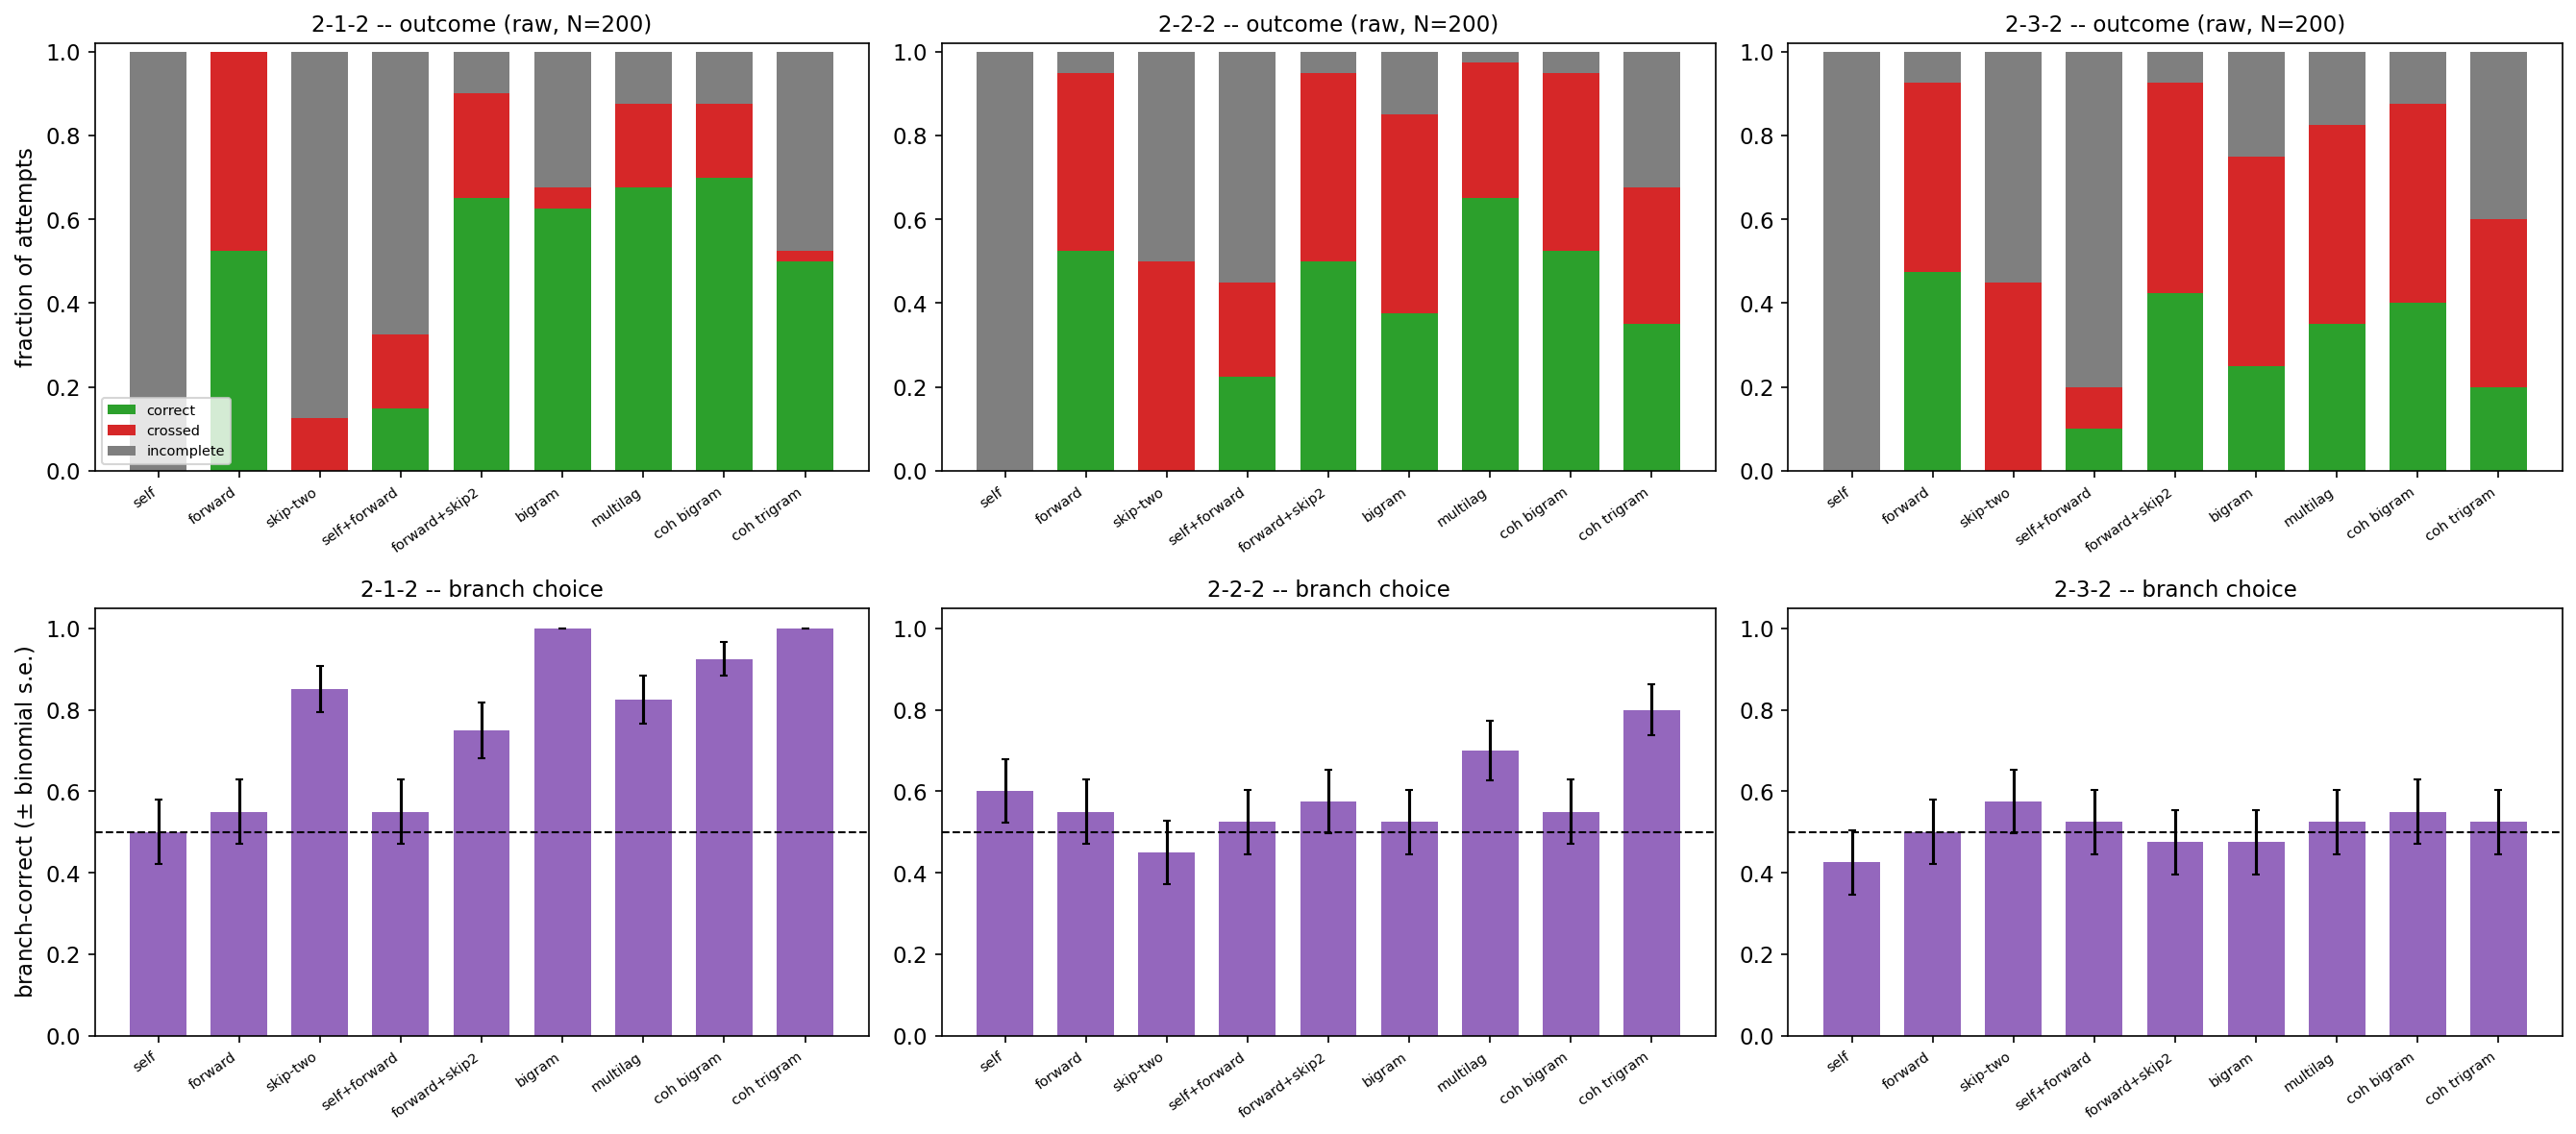
\includegraphics[width=\textwidth,height=0.68\textheight,keepaspectratio]{figures/fig04_benchmark.png}
  \figtitle{Outcome split and branch-correct rate by rule across crossover geometries}
  {\scriptsize Top: outcome split. Bottom: branch choice, $\pm$ binomial standard error
  $\sqrt{p(1-p)/n}$. Dashed line $=$ chance.}
\end{frame}

\begin{frame}{3. Branch choice improves with network size}
  \centering
  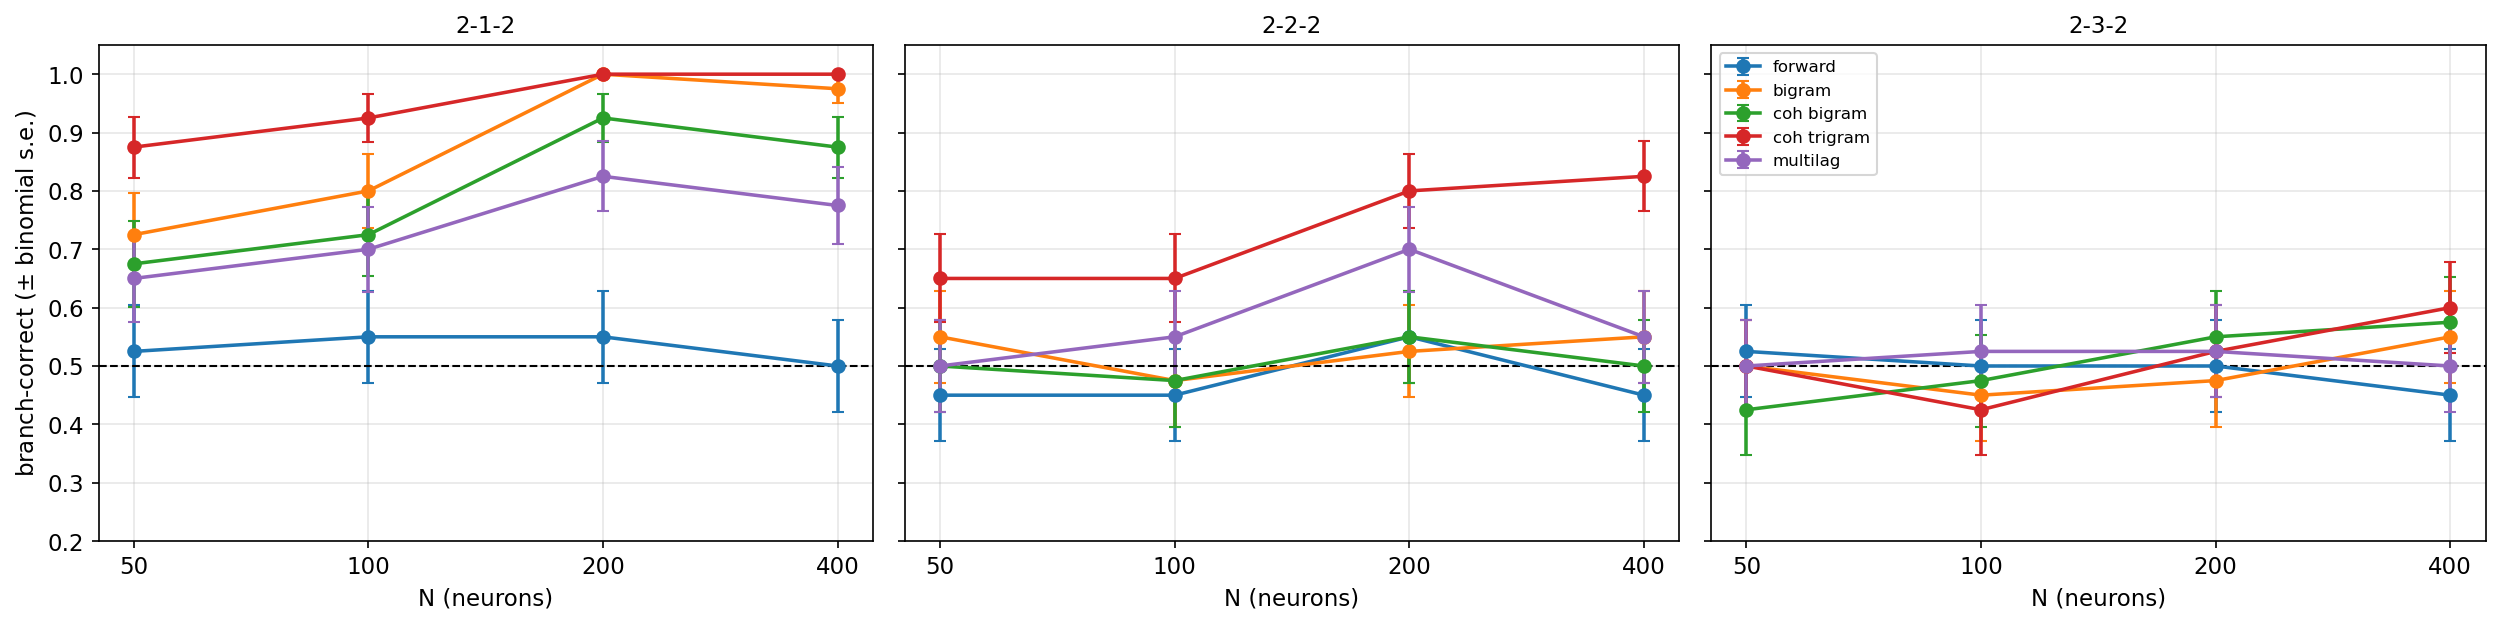
\includegraphics[width=0.96\textwidth,height=0.52\textheight,keepaspectratio]{figures/fig05_branch_vs_N.png}
  \figtitle{Branch-correct rate against network size $N$ on \texttt{2-1-2}}
  \begin{itemize}\small
    \item On \texttt{2-1-2}, branch-correct rises sharply to $N = 200$:
      \texttt{bigram} $80 \to 100\%$, \texttt{coh trigram} $92 \to 100\%$,
      \texttt{coh bigram} $72 \to 92\%$, \texttt{multilag} $70 \to 82\%$.
      $N = 400$ is equal or slightly worse, so $N = 200$ is the operating point.
    \item \textbf{The control works:} \texttt{forward} stays at chance
      ($55 \to 55 \to 50\%$). Network size does not manufacture branch information
      where the gate has none --- the gain is not a decoder artifact.
    \item \textbf{Across $N$, read branch-correct}: at fixed duration
      \texttt{incomplete} rises with $N$ (a larger network needs longer to traverse), so
      \texttt{correct} understates the gain.
  \end{itemize}
\end{frame}

\begin{frame}{3. One hundred instances, with statistics}
  \centering
  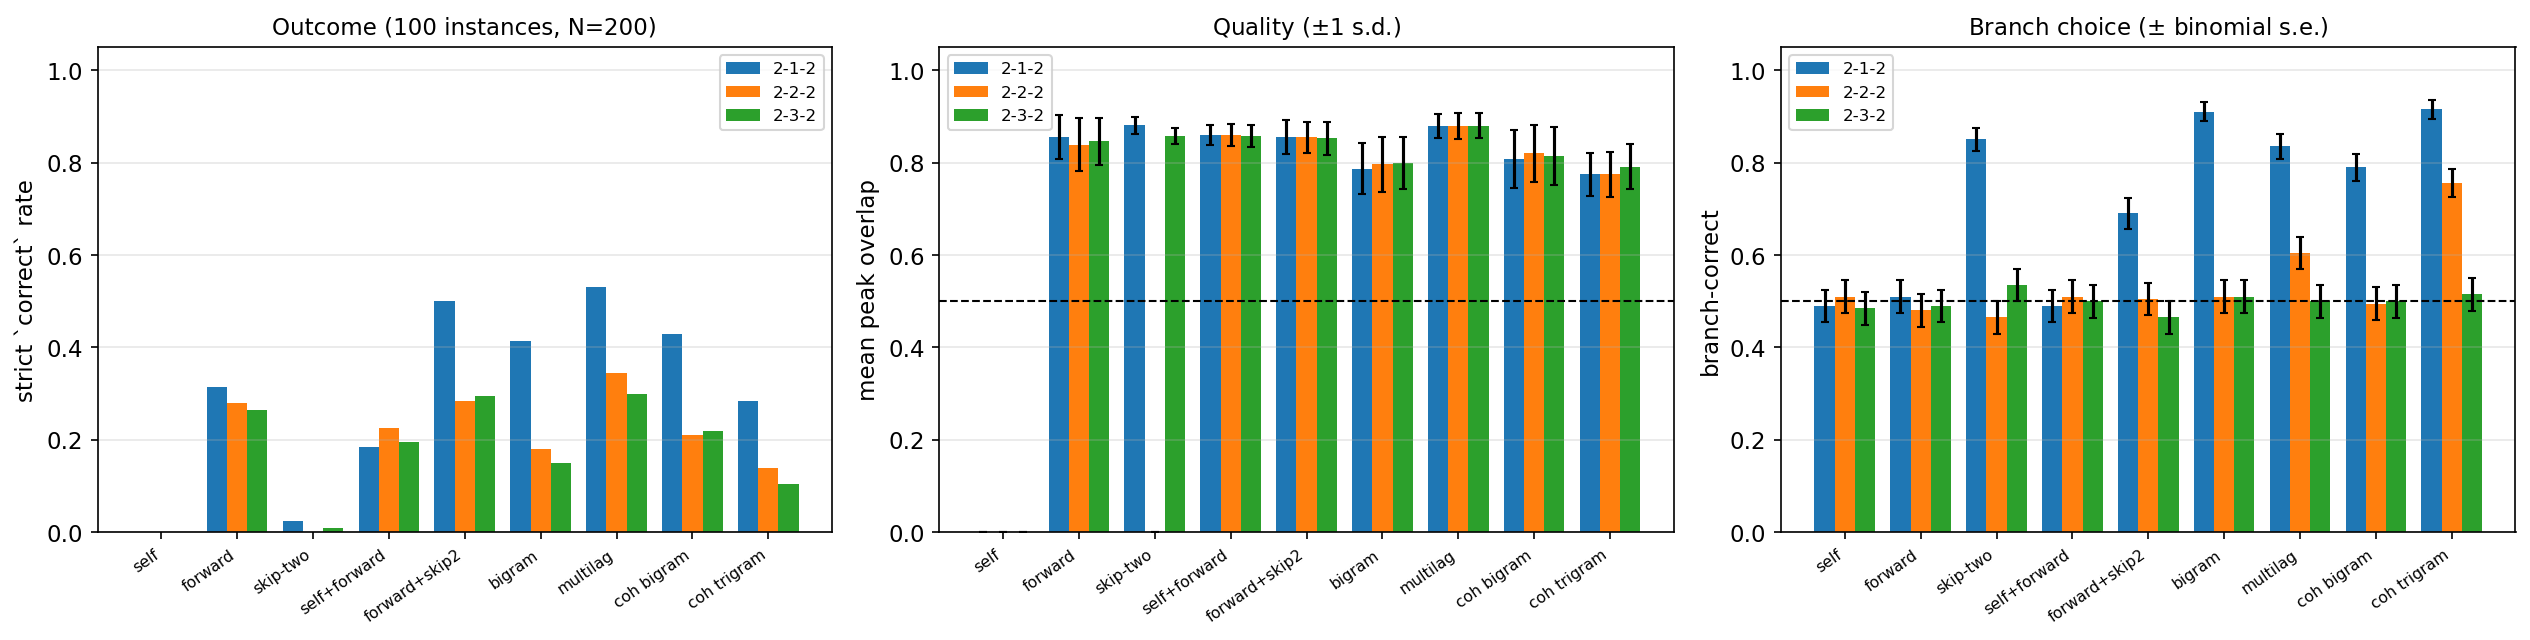
\includegraphics[width=\textwidth,height=0.56\textheight,keepaspectratio]{figures/fig06_seed_sweep.png}
  \figtitle{Retrieval quality and branch choice over $100$ crossover instances per rule}
  {\scriptsize $100$ crossover instances per rule, corruption rate drawn per trial from
  $U[0.12,0.28]$ so each rule faces a range of difficulties; identical instances across rules.
  Error bars: $1$ s.d.\ (quality), binomial s.e.\ (branch choice).}
\end{frame}

\begin{frame}{3. Which rule performs better}
  \centering\footnotesize
  \begin{tabular}{llp{6.6cm}}
    \toprule
    rule & reach & verdict \\
    \midrule
    \texttt{coh trigram} & $2$ & Only rule above chance at $L = 2$; leads
      at $L = 1$. Drawback is the lowest raw drive, which can be fixed with Proportional Gain. \\
    \texttt{coh bigram}, \texttt{bigram} & $1$ & strong at $L = 1$, \textbf{fall to chance at
      $L = 2$} --- the reach prediction, cleanly confirmed. \\
    \texttt{multilag} & $1\ (\times 3)$ & smooth overlap evolution; drive redundancy makes it degrade gracefully. \\
    \texttt{forward} & $0$ & the control. At chance everywhere: its gate reads only the
      shared pattern. \\
    \bottomrule
  \end{tabular}
  \\[3mm]
  \begin{itemize}\small
    \item \textbf{Nothing clears chance on \texttt{2-3-2}} ($L = 3$): every rule reads at most
      two patterns back, so at the branch point every gate factor is still inside the shared run.
    \item \textbf{Reach $\ge L$ only buys a chance.} The discriminating signal is a dynamic
      residual surviving $\sim 2$ steps. Reach is cheap to build; the information is what runs out.
  \end{itemize}
\end{frame}

% ---------------------------------------------------------------- 4
\begin{frame}{4. Robustness: Reading the single-chain metrics}
  \begin{itemize}\small
    \item The crossover metrics do not carry over. On a single chain of $P = 10$:
      \textbf{retrieval fraction} (how much \emph{of a} sequence came back, partial credit)
      vs.\ \textbf{strict rate} (how many \emph{of the} sequences came back whole).
    \item \textbf{The $1/P$ floor.} Position $0$ is the cue and is counted, so nothing scores
      below $10\%$ and a rule that does nothing scores exactly that.
    \item \textbf{\texttt{self} is plotted as a control throughout.} It has no forward
      drive, so its curve \emph{is} the artifact floor: any rule not clearly above it has not
      been shown to retrieve.
    \item \textbf{Robustness sweeps:} performance against network size $N$ and corruption ratio $\rho$, and two knobs on the drive: proportional gain and natural frequency $\omega$.
  \end{itemize}
\end{frame}

\begin{frame}{4. A retracted result: retrieval against $N$}
  \centering
  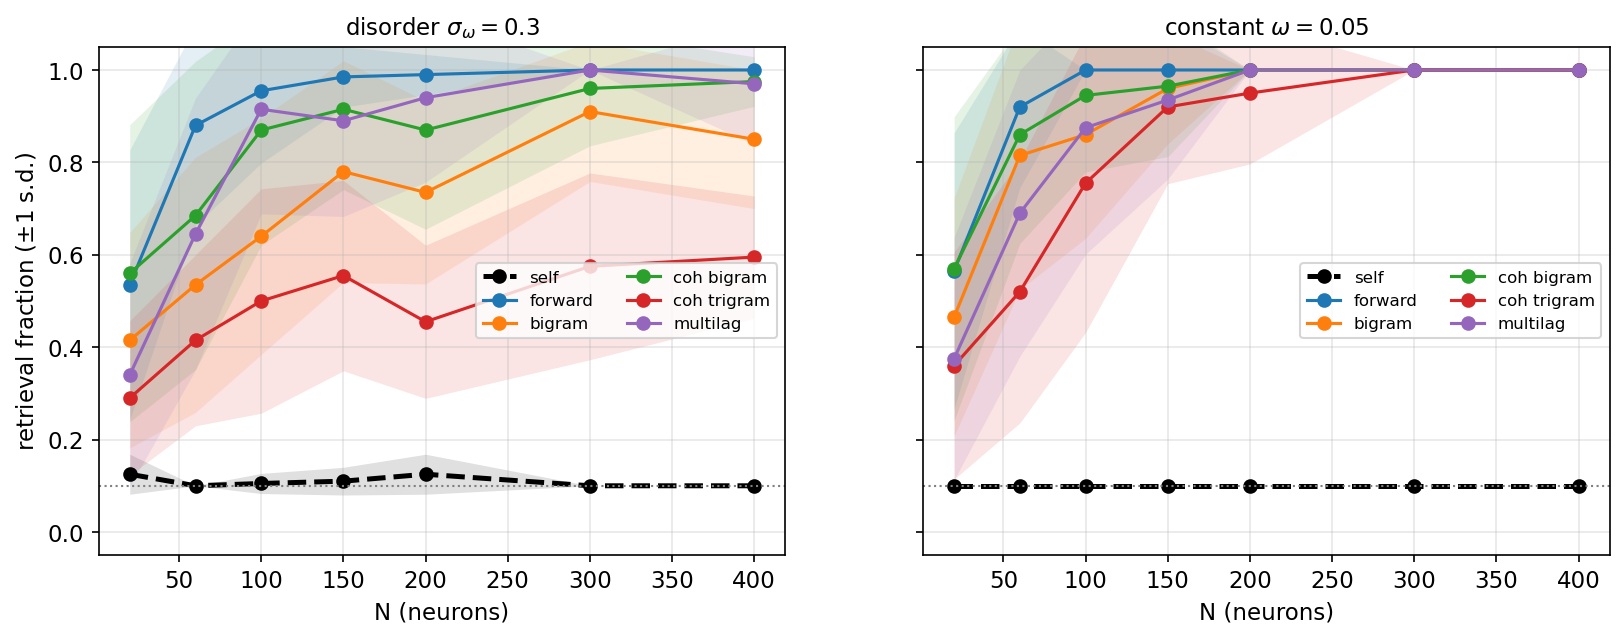
\includegraphics[width=\textwidth,height=0.33\textheight,keepaspectratio]{figures/fig07_N_sweep.png}
  \figtitle{Retrieval fraction against network size $N$ at $T = 180$, heterogeneous and constant $\omega$}
  \begin{itemize}\small
    \item Dip in performance at $N = 200$, most likely associated with scaling of the Lyapunov landscape. This result contradicts with the exponential behavior of \textbf{Krotov's DAM} model. 
    \item $\Delta$ retrieval fraction, $N: 100 \to 400$ --- \texttt{bigram} $+0.21$ (disorder)
      $/ +0.14$ (const.\ $\omega$); \texttt{coh trigram} $+0.09 / +0.24$;
      \texttt{coh bigram} $+0.11 / +0.06$; \texttt{self} (control) $-0.01 / +0.00$.
    \item However, overall retrieval \emph{improves} with $N$; more paterns are stored without crosstalk and interference.
  \end{itemize}
\end{frame}

\begin{frame}{4b. U-shaped dependence on the corruption ratio}
  \centering
  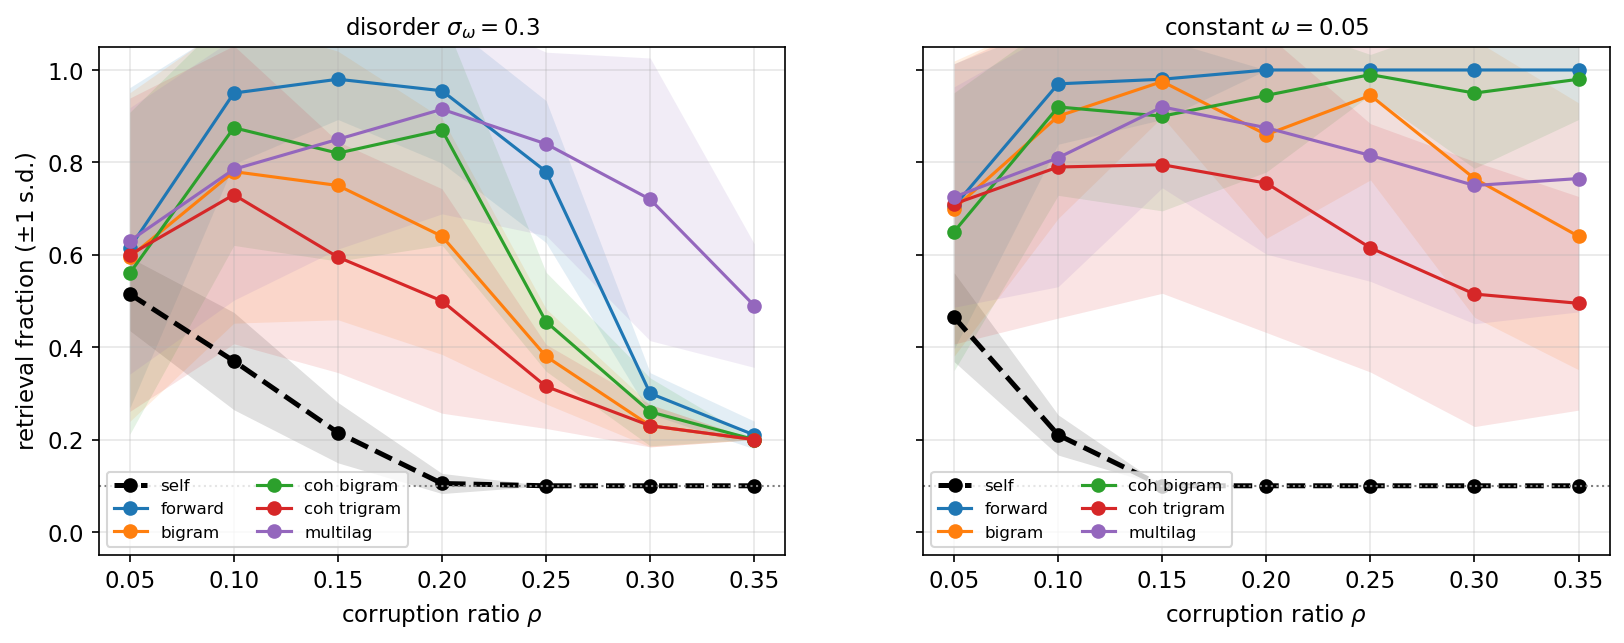
\includegraphics[width=\textwidth,height=0.39\textheight,keepaspectratio]{figures/fig08_rho_U.png}
  \figtitle{Retrieval fraction against corruption ratio $\rho$, heterogeneous and constant $\omega$}
  \begin{itemize}\small
    \item This one \textbf{holds}, in both regimes: an interior peak at
      $\rho \approx 0.10$--$0.25$ with failure at both ends. Small $\rho$: near-duplicates the
      decoder cannot separate. Large $\rho$: consecutive overlaps too small to sustain the cascade.
    \item \textbf{The low end inflates scores.} \texttt{self} peaks at the
      \emph{edge}, $\rho = 0.05$, at $\sim 0.5$ against its $0.10$ floor --- pure artifact.
    \item \textbf{The high end is regime-dependent.} Under disorder it collapses to the floor
      ($\rho = 0.35$: \texttt{forward} $0.21$, \texttt{bigram} $0.20$); at constant $\omega$ it
      barely falls (\texttt{forward} $1.00$, \texttt{coh bigram} $0.98$). So the right-hand
      failure is mostly about the \emph{spread} of $\omega$.
  \end{itemize}
\end{frame}



% ---------------------------------------------------------------- 5
\begin{frame}{5. Appendix: random patterns, and settle vs.\ loop}
  \centering
  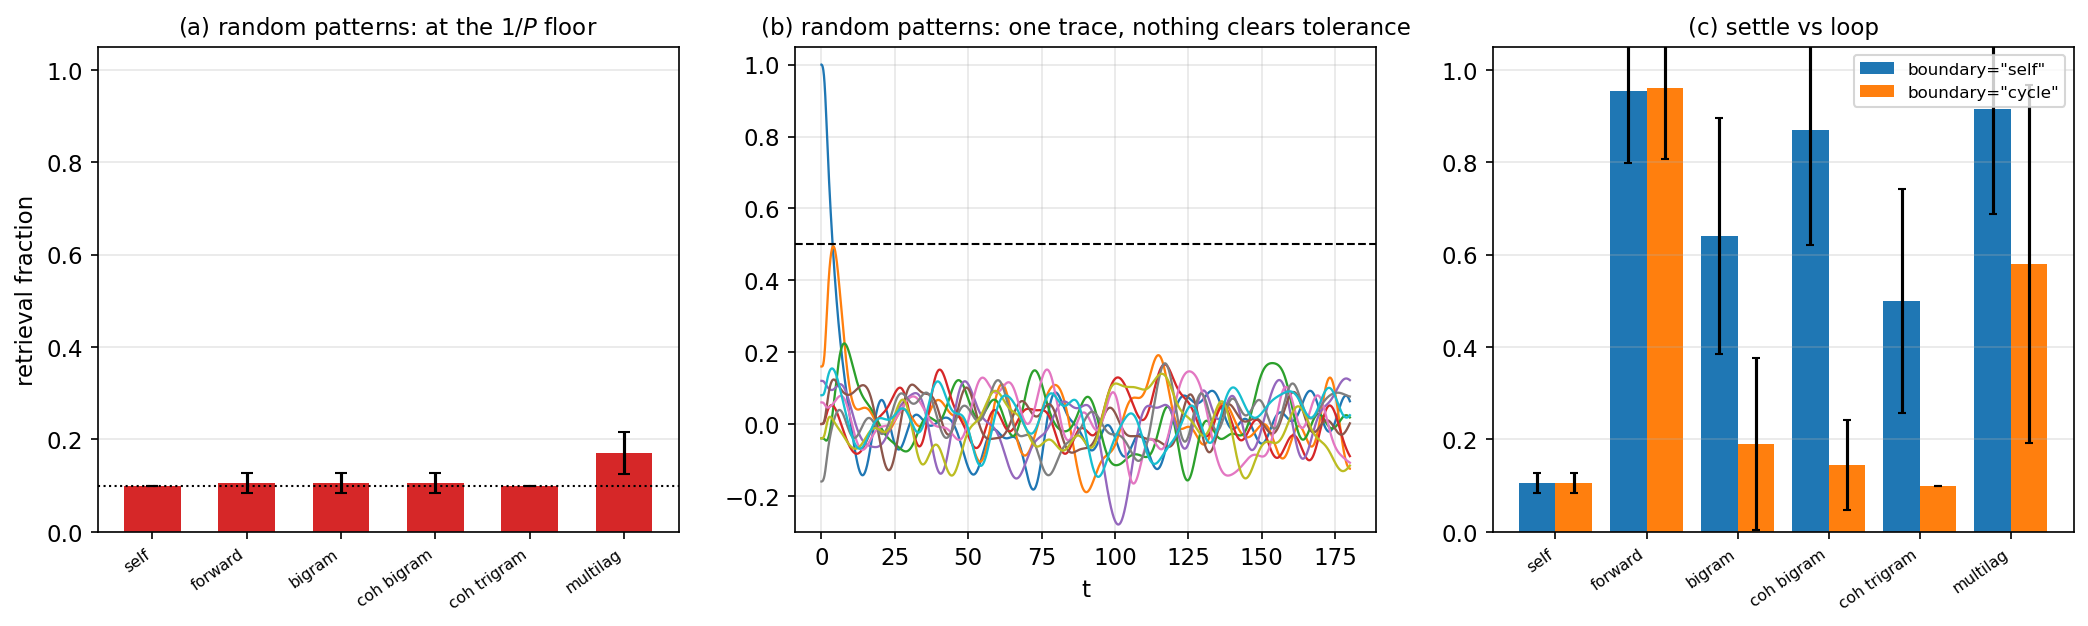
\includegraphics[width=\textwidth,height=0.44\textheight,keepaspectratio]{figures/fig09_appendix.png}
  \figtitle{Controls: independently random patterns (a,b) and \texttt{boundary="cycle"} (c)}
  \begin{itemize}\small
    \item \textbf{(a,b) Random patterns.} Replace the mutation chain with independently random
      patterns and retrieval disappears for \emph{every} rule --- all at the $1/P$ floor, with
      peak overlaps far below \texttt{tolerance}. Sequential similarity structure is a
      prerequisite.
    \item \textbf{(c) \texttt{boundary="cycle"} does not work.} Settling is what makes each
      pattern a usable attractor long enough to be decoded. Wiring the
      last pattern back to the first removes the terminal fixed point and the trajectory
      degrades rather than looping.
  \end{itemize}
\end{frame}

% ---------------------------------------------------------------- findings
\begin{frame}{Findings I: learning rules}
  \begin{itemize}\small
    \item \textbf{Reach $\ge L$ only buys a chance.} The discriminating signal is a
      \emph{dynamic residual} between traversed and untraversed predecessor; it decays within
      $\sim 2$ steps. Reach is cheap to build --- the information is what runs out.
    \item \textbf{\texttt{coh trigram} is the best rule by branch choice}, the only one above
      chance at $L = 2$; \texttt{bigram}/\texttt{coh bigram} hold at $L = 1$ and fall to chance
      at $L = 2$, exactly as reach predicts; \texttt{multilag} is the most robust.
    \item \textbf{Commitment against branch information} is the governing trade-off: lagged
      factors leave fewer for self-amplification, which is why \texttt{correct} and
      \texttt{branch-correct} rank the rules differently.
    \item \textbf{Gain correction cuts both ways:} it recovers the hardest geometry while
      destabilising rules that already succeeded.
    \item \textbf{No rule resolves $L \gtrsim 3$}, and uncorrelated random patterns give the
      floor for \emph{every} rule.
  \end{itemize}
\end{frame}

\begin{frame}{Findings II: dynamics and scaling}
  \begin{itemize}\small
    \item \textbf{A natural frequency is structurally necessary.} At $\omega \equiv 0$ an exact
      cue satisfies $\sin\thetavar_i = 0$: the drive vanishes identically and the system sits at
      an exact fixed point. Because the drive is anchored to the absolute $\{0,\pi\}$ lattice, a
      uniform $\omega$ is a real parameter that no rotating frame removes. The usable band
      $\approx [0.02,0.2]$ is flat --- more $\omega$ buys nothing.
    \item \textbf{Retrieval improves with $N$, like the dense memory it is built on,} and
      branch choice improves markedly with it. The earlier claim that these rules degrade with
      $N$ was an \emph{integration-time artifact} and is withdrawn.
    \item \textbf{U-shaped dependence on $\rho$}: interior peak. The
      high-$\rho$ collapse is mostly the \emph{spread} of $\omega$ and nearly vanishes at
      constant $\omega$; the low-$\rho$ end \emph{inflates} scores rather than depressing them.
    \item \textbf{A low \texttt{correct} is two failures multiplying},
      $\text{correct} \approx \text{branch-correct}\times(1-\text{incomplete})$. The
      \texttt{incomplete} half is a settling problem: the trajectory has parked at a
      sub-tolerance fixed point, and $5\times$ the time does not move it.
    \item \textbf{Integration time is not a free parameter.} A duration validated at one $N$ is
      not validated at another --- the single easiest way to manufacture a false finding here.
  \end{itemize}
\end{frame}


\section[Analysis]{Theoretical Analysis}
% =====================================================================

\begin{frame}{Tensor structure: symmetric vs.\ asymmetric}
  \begin{itemize}
    \item \TODO{write the coupling as $J_i^{\mu_1\dots\mu_d,\nu}$ and split
      it under permutation of the read indices}
    \item \TODO{forward rule $=$ fully symmetric (pure-power) part;
      lag-context rules $=$ mixed-symmetry part}
    \item \TODO{what the decomposition yields: stability conditions, or a
      clean statement of the reach requirement}
  \end{itemize}
\end{frame}

\begin{frame}{Scalability}
  \begin{itemize}
    \item \TODO{cost per step: $\mathcal{O}(KPN)$ buffer $+$
      $\mathcal{O}(\text{terms}\times N)$ drive}
    \item \TODO{capacity in $N$, $d$ --- do context terms cost capacity?}
    \item \TODO{Jona: scaling law / bound}
  \end{itemize}
\end{frame}


% =====================================================================
\section[Conclusions]{Conclusions and Outlook}
% =====================================================================

\begin{frame}{Conclusions}
  \begin{block}{Main result}
    To resolve branching after a shared segment, the learning rule needs a
    \textbf{lag reference exceeding the length of the shared segment.} Only a
    factor reading back past the last shared pattern breaks the innate
    symmetry of the Lyapunov function; rules whose lags all sit inside the
    shared run are symmetric in the branches by construction.
  \end{block}
  \begin{itemize}
    \item Markov-1 Kuramoto DAM retrieves single sequences reliably, but its
      Lyapunov function is symmetric at every shared state, leaving the
      branch choice to noise.
    \item Sufficient reach is only the entry ticket: commitment and
      branch information trade off.
    \item The rule alone does not fix the operating point: $\rho$, $N$ and
      $\sigma_\omega$ set it \emph{together}.
  \end{itemize}
\end{frame}

\begin{frame}{Applications}
  \begin{itemize}
    \item \textbf{Physical simulators.} Every rule is pure oscillator
      coupling, and therefore maps onto analog and photonic Kuramoto
      hardware: crossover-resolving memory as a physical primitive.
    \item \textbf{Neurobiology.} \TODO{phase-coded replay, theta--gamma;
      lag-context gating as a disambiguation mechanism}
    \item \TODO{motor-sequence chaining, time-series disambiguation}
  \end{itemize}
\end{frame}


% =====================================================================
\section[Open Questions]{Active Questions for Further Investigation}
% =====================================================================

\begin{frame}{Active questions}
  \begin{enumerate}
    \item How are these learning rules implemented in \textbf{physical
      (oscillator-based) simulators}?
    \item What is the role of \textbf{decaying neurons}, and can they
      replace the explicit lag buffer?
    \item How does one generate \textbf{robust rules for randomly generated
      pattern sequences}?
  \end{enumerate}
  \vspace{3mm}
  {\small Further open questions: whether the resolvable shared-run length
  $L$ admits a fundamental ceiling, and whether rule weights can be
  \emph{learned} rather than constructed by hand.}
\end{frame}

\begin{frame}{Question 1: physical implementation}
  \begin{itemize}
    \item Rules are rank-$(d{+}1)$ couplings; hardware (Ising machines, OPO
      and polariton networks, CMOS oscillatory NNs) gives \emph{pairwise}.
      Which mechanism synthesizes the product: ancilla modes, parametric
      mixing, or measurement feedback?
    \item Can the lagged factor $\mvar_{\mu-\ell}$ be a physical \emph{delay
      line} rather than a stored buffer? This would render the rule local
      in time as well as in space.
    \item \TODO{required coupling precision and noise floor before branch
      choice falls to chance}
  \end{itemize}
\end{frame}

\begin{frame}{Question 2: decaying neurons}
  \begin{itemize}
    \item Replace the discrete lag by a decaying trace
      $\tau \dot h_\mu = -h_\mu + |\mvar_\mu|^2$. Adaptation achieves the same
      from the opposite direction: the active pattern suppresses itself and
      releases the flow to its successor.
    \item Open: whether a single time constant $\tau$ provides reach beyond
      the shared segment, and whether it is simpler to realize physically
      than a multi-lag product.
  \end{itemize}
  \begin{block}{Selected references}
    \footnotesize
    \textbf{Delayed / slow synapses:} Sompolinsky \& Kanter (PRL 57, 2861,
    1986); Kleinfeld (PNAS 83, 9469, 1986); Tank \& Hopfield (PNAS 84, 1896,
    1987).
    \textbf{Adaptation-driven transitions:} Horn \& Usher (Phys.\ Rev.\ A 40,
    1036, 1989); Herrmann, Ruppin \& Usher (Biol.\ Cybern.\ 68, 455, 1993);
    Treves (Cogn.\ Neuropsych.\ 22, 276, 2005) --- latching; Recanatesi et
    al.\ (Front.\ Comput.\ Neurosci.\ 9:149, 2015); Gillett, Pereira \&
    Brunel (PNAS 117, 29948, 2020).
    \textbf{Closest precedent:} Martinez Mayorquin et al.\ (ICANN 2019,
    pp.\ 793--805) --- filtered synaptic traces for \emph{sequence
    disambiguation}.
  \end{block}
\end{frame}

\begin{frame}{Question 3: randomly generated sequences}
  \begin{itemize}
    \item Uncorrelated patterns: $0\%$ retrieval for every rule, raw and
      gain-corrected --- peak overlaps $0.16$--$0.19$ against a $0.5$
      tolerance.
    \item The gate fails before the drive does: for independent patterns
      $\mvar_{\mu-\ell} = \mathcal{O}(N^{-1/2})$; rescaling a gate that reads
      $\mvar \approx 0$ has no effect.
    \item To test: whitened / pseudo-inverse storage (Chaudhry et al.,
      \emph{Long Sequence Hopfield Memory}); larger $d$; ridge-fitted
      weights as an upper-bound control.
    \item \TODO{retrieval rate vs.\ pattern correlation, mutation chain
      $\to$ fully random: locate the collapse threshold per rule}
  \end{itemize}
\end{frame}

\begin{frame}
  \centering
  \Large Thank you \\[2mm]
  \normalsize \TODO{ repo QR}
\end{frame}

\end{document}



